\section{数据集制作流程}

不同源光学影像超分数据集制作流程如图\ref{fig:0101}所示:

\begin{figure}[htbp]
    \centering
    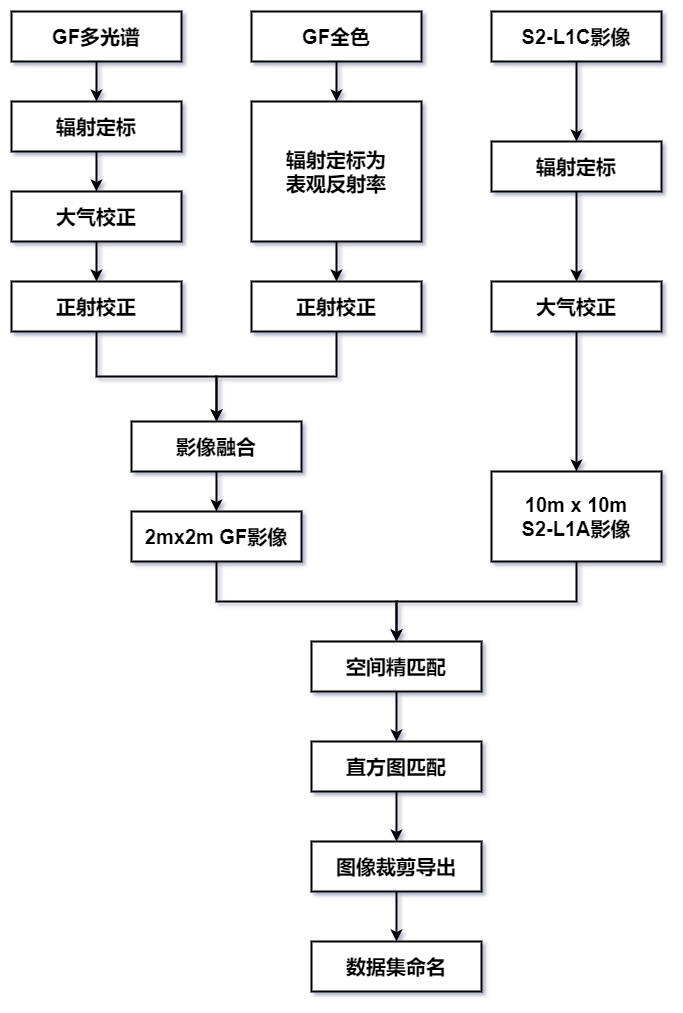
\includegraphics[height=0.7\textheight]{pic/cha01.png}
    \caption{整体流程图}
    \label{fig:0101}
\end{figure}

为了得到高分辨率光学影像, 需要对高分数据进行融合. 在对高分多光谱数据进行辐射定标, 大气校正, 正射校正后, 得到预处理后分辨率为8m x 8m的光学遥感影像; 之后对全色影像进行辐射定标和正射校正, 得到预处理后分辨率为2m x 2m的全色影像. 注意, 全色影像没有大气校正, 所以一般在定量遥感中不使用全色影像. 为提高影像融合速度(4倍左右), 将多光谱数据的储存顺序由BSQ转为BIP, 之后使用NND(Nearest Neighbor Diffusion)影像融合方法进行影像融合, 得到分辨率为2m x 2m的遥感光学影像.

哨兵2号L1C级数据已经进行过正射校正, 因此只需要使用欧空局提供的Sen2Cor即可完成哨兵数据的辐射定标和大气校正, 得到预处理后分辨率为10m x 10m 的L1A级光学遥感影像. 

由于遥感数据不同源, 同一地物在不同源影像中位置不同,  因此需要对遥感影像进行精细匹配; 超分数据要求图像色彩一致, 因此在进行空间精匹配后, 需要进行影像直方图匹配. 

本次实验中使用的高分影像为2020年04月xx日PMS的多光谱影像作为炒粉数据中的高分辨率影像; 使用的哨兵数据为2020年04月xx日的影像作为超分数据集中的低分辨率影像. 理论上, 制作的超分影像数据集覆盖区域为广东省xx市. 使用的原始遥感影像编号分别为:
\begin{itemize}
    \item xxxxxxxxxxxxxxxxxxxxxxxxxxxxxxxxxxxx
    \item xxxxxxxxxxxxxxxxxxxxxxxxxxxxxxxxxxxx
\end{itemize}

思考问题:
\begin{itemize}
    \item 为何不同源影像同一地物位置会存在一定偏差
    \item 为何BIL数据顺序更适合影像融合
\end{itemize}

